%\documentclass[12pt]{report}
%
%% some macros
%% Here, you can define your own macros. Some examples are given below.

\newcommand{\R}[0]{\mathds{R}} % real numbers
\newcommand{\Z}[0]{\mathds{Z}} % integers
\newcommand{\N}[0]{\mathds{N}} % natural numbers
\newcommand{\C}[0]{\mathds{C}} % complex numbers
\newcommand{\bm}[1]{{\boldsymbol{{#1}}}} % vector
\newcommand{\mat}[1]{{\boldsymbol{{#1}}}} % matrix

\newcommand{\E}[1]{\mathbb{E}_{#1}} % Expectation
\newcommand{\Pd}[1]{\mathbb{P}_{#1}} % Probability Distribution

%%%%%%%%%%%%%%%%%%%%%%%%%%%%%%%%%%%%%%%%%%
% University Assignment Title Page 
% LaTeX Template
% Version 1.0 (27/12/12)
%
% This template has been downloaded from:
%%%%%%%%%%%%%%%%%%%%%%%%%%%%%%%%%%%%%%%%%
%----------------------------------------------------------------------------------------
%	PACKAGES AND OTHER DOCUMENT CONFIGURATIONS
%----------------------------------------------------------------------------------------

\usepackage[nottoc,notlot,notlof]{tocbibind}
\usepackage[T1]{fontenc}
%\usepackage{hyperref}
\usepackage{indentfirst}
\usepackage{amsmath}
\usepackage{amssymb}
\usepackage{graphicx}
\usepackage{subcaption}
\usepackage{geometry}
 \geometry
 {
     a4paper,
     left=25mm,
     right=25mm,
     top=30mm,
     bottom=30mm,
 }

% \usepackage[a4paper,hmargin=2.8cm,vmargin=2.0cm,includeheadfoot]{geometry}
\usepackage{textpos}
\usepackage{natbib} % for bibliography
%\usepackage{tabularx,longtable,multirow,subfigure,caption}
\usepackage{fncylab} %formatting of labels
\usepackage{fancyhdr} % page layout
\usepackage{url} % URLs
\usepackage[english]{babel}
%\usepackage{dsfont}
\usepackage{epstopdf}
\usepackage{backref} % needed for citations
\usepackage{array}
\usepackage{latexsym}
\usepackage[pdftex,pagebackref,hypertexnames=false,colorlinks]{hyperref} % provide links in pdf
 
\hypersetup{pdftitle={},
  pdfsubject={}, 
  pdfauthor={},
  pdfkeywords={}, 
  pdfstartview=FitH,
  pdfpagemode={UseOutlines},% None, FullScreen, UseOutlines
  bookmarksnumbered=true, bookmarksopen=true, colorlinks,
    citecolor=black,%
    filecolor=black,%
    linkcolor=black,%
    urlcolor=black}
 
\usepackage[all]{hypcap}
\frenchspacing

\DeclareMathOperator{\tr}{tr}
%
%\begin{document}

\externaldocument{lit_review}
\externaldocument{facial_modelling_background}
\externaldocument{appendix}

\chapter{Blendshape Classification}

This chapter shall discuss the problem of word level classification from blendshape parameters obtained from a dataset created with the VOCA model \cite{Cudeiro2019} processing audio from the LRW dataset \cite{Chung2016}.
Classification is performed with a Convolutional Neural Network architecture on 500 labels.
The model architecture, how performance is assessed and how the model has been tuned to maximise performance on a held out validation set is also discussed. 

\section{Problem Definition}
As with traditional lip reading problems, the end goal of VSR models using 3D temporal data is to correctly classify variable length input sequences at a sentence level.
However, before this problem can be tackled, the simpler problem of word level classification should be first approached to ensure that this is possible, before moving on to more advanced problems.
If word level classification cannot be achieved, it may be concluded that there is not a sufficient amount of information encoded in 3D temporal models for more complex problems to be solved with the current set of assumptions.

These assumptions include:
\begin{enumerate}
    \item Provided an appropriate dataset of 3D temporal facial scans of subjects speaking, a set of blendshape parameters which realistically represent the motions of speech can be found. \label{assumption:class_1}
    \item The blendshape parameters represent an encoding from which a classification model is able to make word level predictions from. \label{assumption:class_2}
\end{enumerate}

\section{Generation of a 3D Lip Reading Dataset}
In order to train any model, an appropriate dataset must exist upon which the model can be trained.
An appropriate dataset for word level prediction from blendshape parameters would consist of:
\begin{itemize}
   \item A large enough vocabulary that single instances of words with unique phonemes do not exist as this would allow classification of these words too simple.
   \item Facial mesh recordings for all samples in the dataset, all of with brought into alignment to remove movement not related to speech.
   \item Principal blendshape axis which can be shown to contain useful interpolation for speech.
   \item The blendshape parameters corresponding to each sample for the given blendshape axis.
\end{itemize}

As discussed in section \ref{3D Datasets}, currently there exists no public datasets which have been created for the purpose of lip reading from 3D temporal data.
In addition to this, the datasets which have not been created with the purpose of lip reading but do contain 3D temporal data of speaking facial scans, are either not public in the case of Karras's model \cite{Karras2017a} or are unlabelled and too small to train a model effectively as is the case with the VOCASET \cite{Cudeiro2019}.
Both of these datasets also contain a large vocabulary, with too few samples of each word.
The VOCASET dataset could be labelled with the use of an automatic speech recognition model such as DeepSpeech as suggested in section \ref{3D Datasets}, however as the dataset was constructed to contain as much variation in speech sounds, so a degree of word repetition would offer little benefit, hence the lack of consistent word repetition.

In order to tackle the issue of an appropriate dataset not existing, two solutions exist.
The ideal solution would be to capture subjects speaking words from a set corpus using a 3D capture equipment, this solution was not a viable option for this project due to the specialised equipment required and the data processing required after data capture had been performed.
Another means of constructing the dataset would be to generate the data with an existing model which can convert an appropriate audio dataset to a series of facial meshes from which blendshape axis can be constructed and parameters recovered.
This can be achieved by processing audio from the LRW dataset \cite{Cheng2016} though the VOCA model \cite{Cudeiro2019}.
The VOCA model claims to be able to generate realistic 3D facial motion from audio, as lip reading is notoriously difficult for humans, this is difficult to validate.
Assuming that the VOCA model does in fact generate realistic facial motion, the LRW dataset allows for a 3D dataset to be generated with a set corpus of the 500 words contained in the LRW dataset.

55,000 audio samples are taken from the LRW dataset with a uniform distribution of all labels, resulting in 110 samples for each label.
Audio samples from the LRW dataset are from ``in the wild'' scenarios \cite{Cheng2016}, meaning that there is background noise and audio in the clip.
An sample of the word ``\textit{ABOUT}'' will contain the word ``\textit{ABOUT}'' within the audio sample, but will contain other speech either side of the clip.
Figure \ref{fig:LRW_About} shows such a sample labelled as ``\textit{ABOUT}'' in which the phrase ``talking about fair'' is spoken.

\begin{figure}[h]
    \centering
        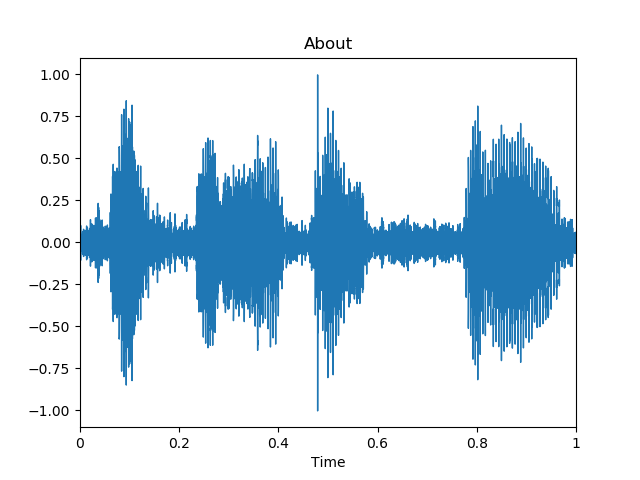
\includegraphics[width=0.7\textwidth]{figures/about.png}
    \caption{Audio Sample from LRW \cite{Cheng2016} ``Talking About Fair''}\label{fig:LRW_About}
\end{figure}

The full LRW dataset contains 1000 training samples for each label, however due to the size of the VOCA model, processing 55000 samples (11\% of the full dataset) took roughly 8 days to process with the GPU acceleration of a Nvidia Tesla M60.
This is due to the size of the VOCA model, which incorporates the DeepSpeech model as a means of audio feature extraction.
In parallel to the generation of the 3D temporal data from the VOCA model, blendshape parameters were recovered as the facial scans were produced.
No significant decrease in speed the speed of data generation was observed running these tasks in parallel.

\subsection{Blendshape Axis Creation}
Ideally, all 55000 samples would be collected and the PCA would be performed on this to construct the blendshape axis.
However, due to disk space limitations a complete dataset of 55000 facial scans could not be collected at once due to the size of the generated facial meshes as this would total 2.365 million generated facial mesh data samples, each of which occupying around 185KB, requiring a total of 440GB of disc space.
To perform PCA on the generated facial meshes for blendshape axis (see section \ref{blendshapes}), the first 5000 facial mesh sequences were generated totalling 83 minutes of data and 215000 individual facial mesh data samples. 
Once PCA has been applied to a dataset of facial scans, the transformation matrix $\mat{W}$ is known.
$\mat{W}$ has columns of eigenvectors corresponding to eigenvalues, each of these eigenvectors represents the principal axis upon which can be interpolated upon.
These axis are the blendshapes axis and by interpolating along these axis by given amounts, motions of the facial mesh can be expressed in a low dimension.
The first blendshape axis corresponds to the largest eigenvalue, as that axis contains the largest amount of variation amongst the dataset.
The number of blendshapes which can be created will be limited by the number of positive non-zero eigenvalues found from PCA, however as each successive blendshape axis corresponds to a decreasingly small eigenvalue, the amount of variation in each successive axis decreases. 
This results in realistic reconstruction being able to be achieved with a relatively small number of blendshapes containing the majority of the variation within the dataset.
Examples of the First and Second Blendshape Axis from the first 5000 samples are shown in Figures \ref{fig:Blendshape_axis_1} and \ref{fig:Blendshape_axis_2} respectively, further examples can be viewed in the Appendix: Figure \ref{fig:Blendshape_axis_3}, \ref{fig:Blendshape_axis_4}.
These are constructed by interpolating along each axis individually by a fixed step amount.

\begin{figure}[h]
    \centering
    \begin{subfigure}[b]{0.24\textwidth}
        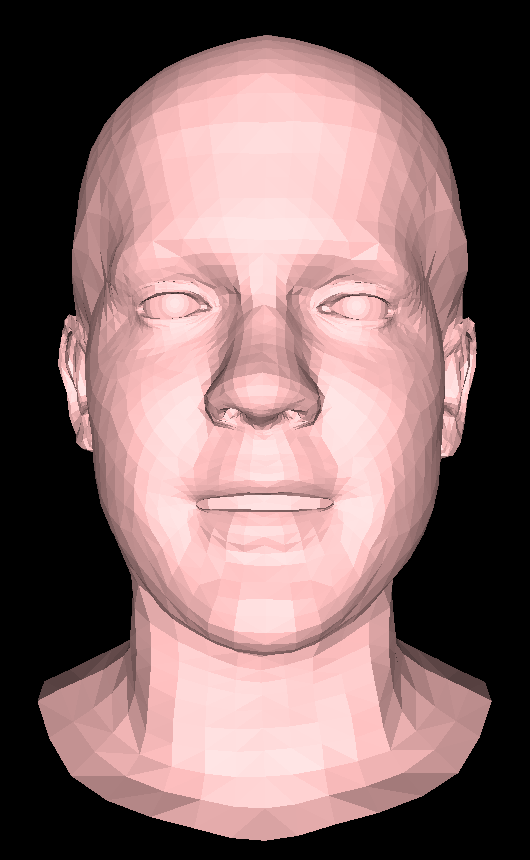
\includegraphics[width=\textwidth]{figures/blendshape_interp/1/00001.png}
    \end{subfigure}
    \begin{subfigure}[b]{0.24\textwidth}
        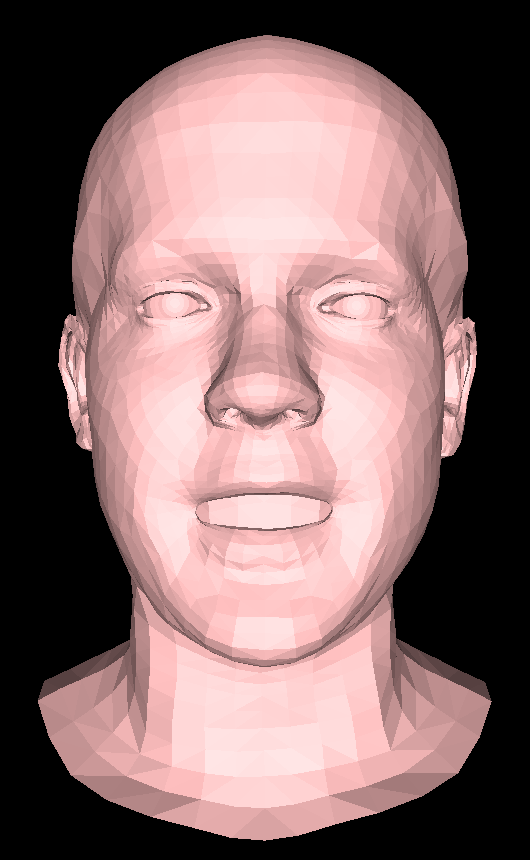
\includegraphics[width=\textwidth]{figures/blendshape_interp/1/00002.png}
    \end{subfigure}
    \begin{subfigure}[b]{0.24\textwidth}
        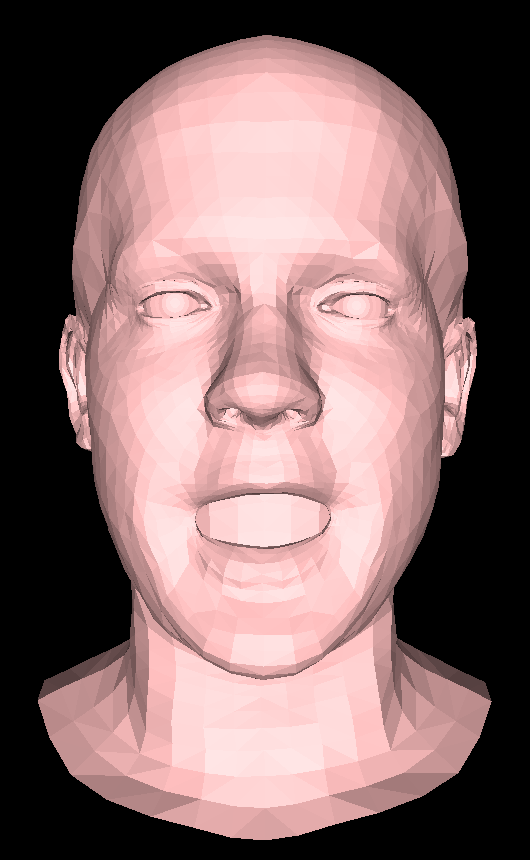
\includegraphics[width=\textwidth]{figures/blendshape_interp/1/00003.png}
    \end{subfigure}
    \begin{subfigure}[b]{0.24\textwidth}
        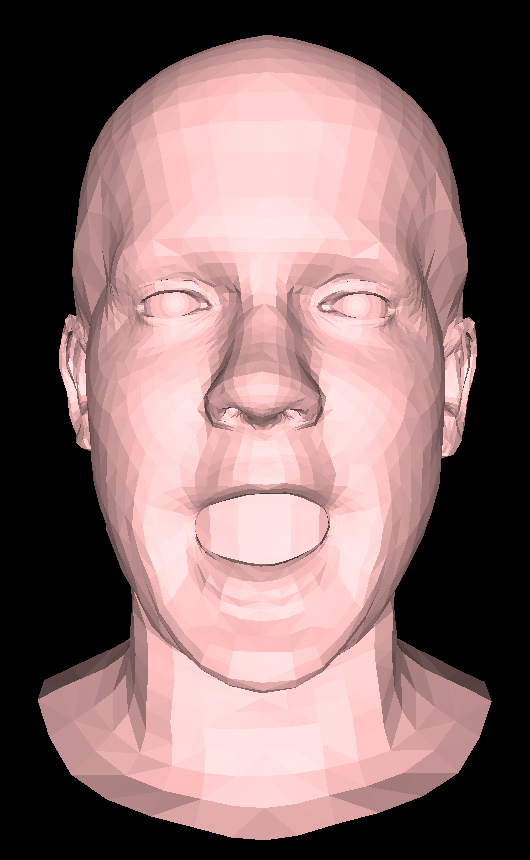
\includegraphics[width=\textwidth]{figures/blendshape_interp/1/00004.png}
    \end{subfigure}
    \caption{First Blendshape Axis Interpolation }\label{fig:Blendshape_axis_1}
\end{figure}
\begin{figure}[h]
    \centering
    \begin{subfigure}[b]{0.24\textwidth}
        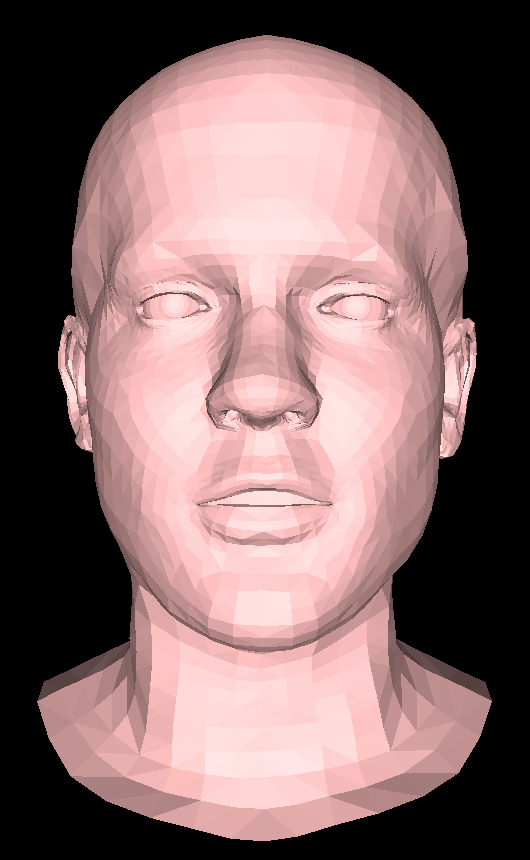
\includegraphics[width=\textwidth]{figures/blendshape_interp/2/00001.png}
    \end{subfigure}
    \begin{subfigure}[b]{0.24\textwidth}
        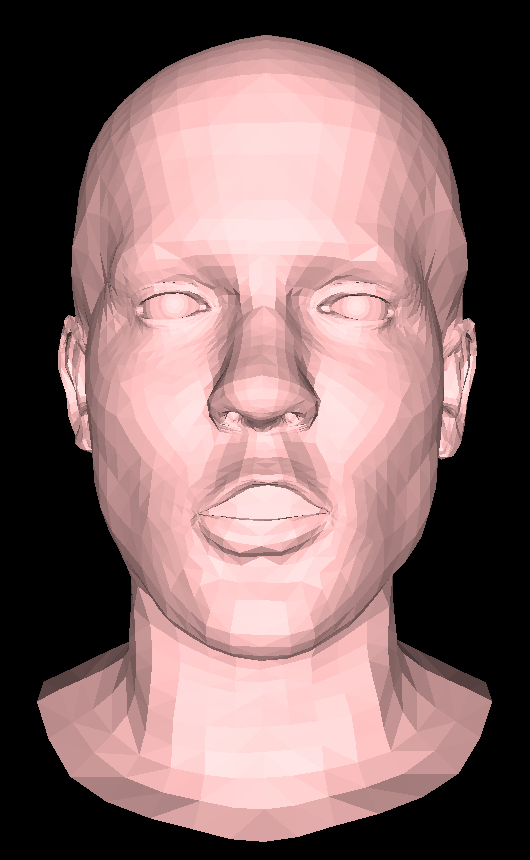
\includegraphics[width=\textwidth]{figures/blendshape_interp/2/00002.png}
    \end{subfigure}
    \begin{subfigure}[b]{0.24\textwidth}
        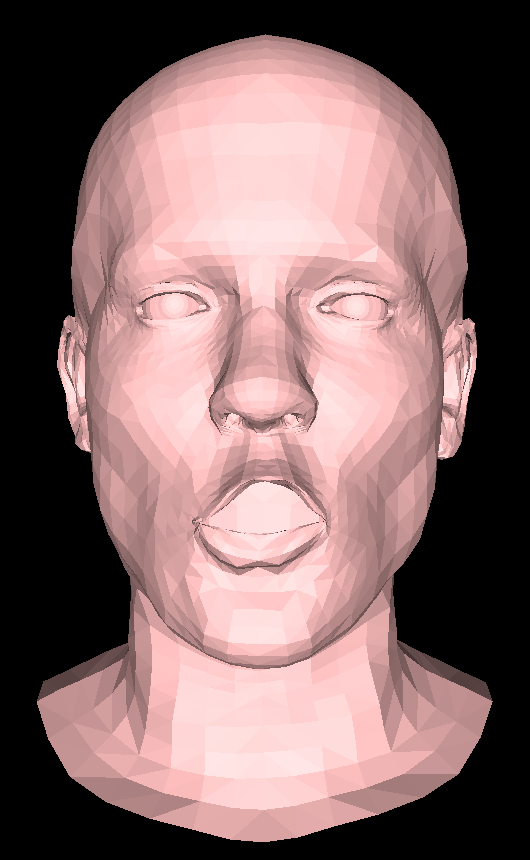
\includegraphics[width=\textwidth]{figures/blendshape_interp/2/00003.png}
    \end{subfigure}
    \begin{subfigure}[b]{0.24\textwidth}
        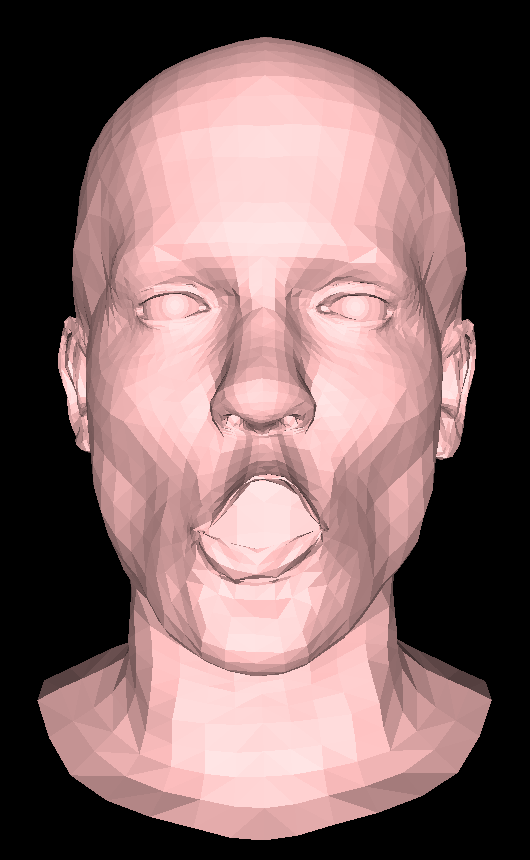
\includegraphics[width=\textwidth]{figures/blendshape_interp/2/00004.png}
    \end{subfigure}
    \caption{Second Blendshape Axis Interpolation}\label{fig:Blendshape_axis_2}
\end{figure}

\subsection{Blendshape Parameter Recovery}
Given a template mesh $\mat{M} \in \mathbb{R}^{(N \times 1)}$ upon which to interpolate from, where $N = 3n$ and $n$ represents the number of vertex points in the facial mesh, each of which have an $x, y$ and $z$ coordinate value and Blendshape Axis $\mat{W} \in \mathbb{R}^{(N \times d)}$ as described in section \ref{sec:pca}, where the $d$ first principal axis have been kept, representing the axis along which the template mesh $\mat{M}$ can be interpolated.

\begin{equation*}
    \mat{M} = \begin{bmatrix} 
                x_{1}, &
                y_{1}, &
                z_{1}, &
                \dots, &
                x_{n}, &
                y_{n}, &
                z_{n}
               \end{bmatrix}^\top,
    \quad
    \mat{M} \in \mathbb{R}^{N\times 1},
    \quad
    N = 3n,
\end{equation*}
\quad
\begin{equation*}
    \mat{W} = [
               \bm{w_1}, \dots, \bm{w_d}
              ],
    \quad
    \mat{W} \in \mathbb{R}^{(N \times d)}
\end{equation*}
\quad
\begin{equation*}
    \bm{w_i} = \begin{bmatrix} 
                x_{1}, &
                y_{1}, &
                z_{1}, &
                \dots, &
                x_{n}, &
                y_{n}, &
                z_{n}
    \end{bmatrix}^\top
\end{equation*}

Given subsequent frames $\mat{M}^{\prime}$ which deviate the facial mesh from $\mat{M}$, $\mat{M}^{\prime}$ can be expressed by equation \ref{eq:mesh_interp}, where $\bm{\Lambda}$ is a vector containing Blendshape parameters.

\begin{equation}\label{eq:mesh_interp}
    \mat{M}^{\prime} = \mat{M} + \mat{W} \mat{\Lambda}
\end{equation}
\quad
\begin{equation*}
    \mat{\Lambda} = \begin{bmatrix}
        \lambda_1, &
        \dots, &
        \lambda_d
    \end{bmatrix}^\top
\end{equation*}

The blendshape parameters $\lambda_i$ can be found by rearranging equation (\ref{eq:mesh_interp}) and solving for $\bm{\Lambda}$ as shown in equation (\ref{eq:mesh_interp_lambda}).
The solution to this can be found by finding the pseudo-inverse for the Blendshape Axis $\mat{W}$.

\begin{equation}\label{eq:mesh_interp_lambda}
    \mat{\Lambda} = \mat{W}^{-1}(\mat{M}^{\prime} - \mat{M})
\end{equation}

\section{Data Preprocessing}
To aid training, the dataset is normalised to a range of [0,1] using equation (\ref{eq:normalise}) where $x_{min}$ and $x_{max}$ are the smallest and largest values in the dataset respectively.
As each Blendshape Axis is unrelated, normalisation is applied separately per axis (Figure \ref{fig:hist_norm}).
This is beneficial as the variance in parameters values decreases from the first axis, as can be seen in Figure \ref{fig:hist_unnorm} the histogram plot of the Blendshape Parameters before normalisation.

\begin{equation} \label{eq:normalise}
   x^\prime = \frac{x - x_{min}}{x_{max} - x_{min}} 
\end{equation}

\begin{figure}[h]
    \centering
    \begin{subfigure}[b]{0.49\textwidth}
        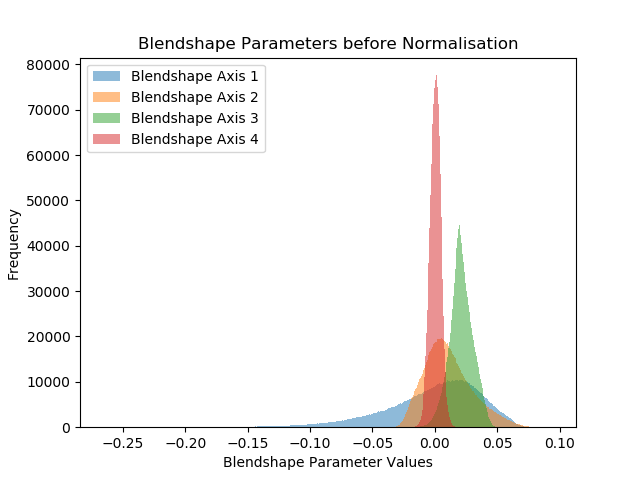
\includegraphics[width=\textwidth]{figures/shape_params_unnormalised_hist.png}
        \caption{Unnormalised}\label{fig:hist_unnorm}
    \end{subfigure}
    \begin{subfigure}[b]{0.49\textwidth}
        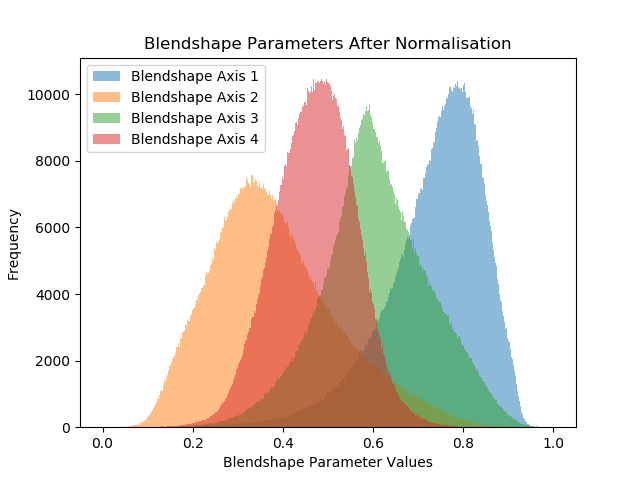
\includegraphics[width=\textwidth]{figures/shape_params_normalised_seperately_hist.png}
        \caption{Normalised}\label{fig:hist_norm}
    \end{subfigure}
    \caption{Blendshape Parameter Histograms}
\end{figure}


\section{Model Architecture}

\section{Results}

\section{Discussion}

%\bibliographystyle{unsrt}
%\bibliography{ref}
%\end{document}